\chapter{Introduction \& Motivation}

\begin{figure}[H]
  \centering
  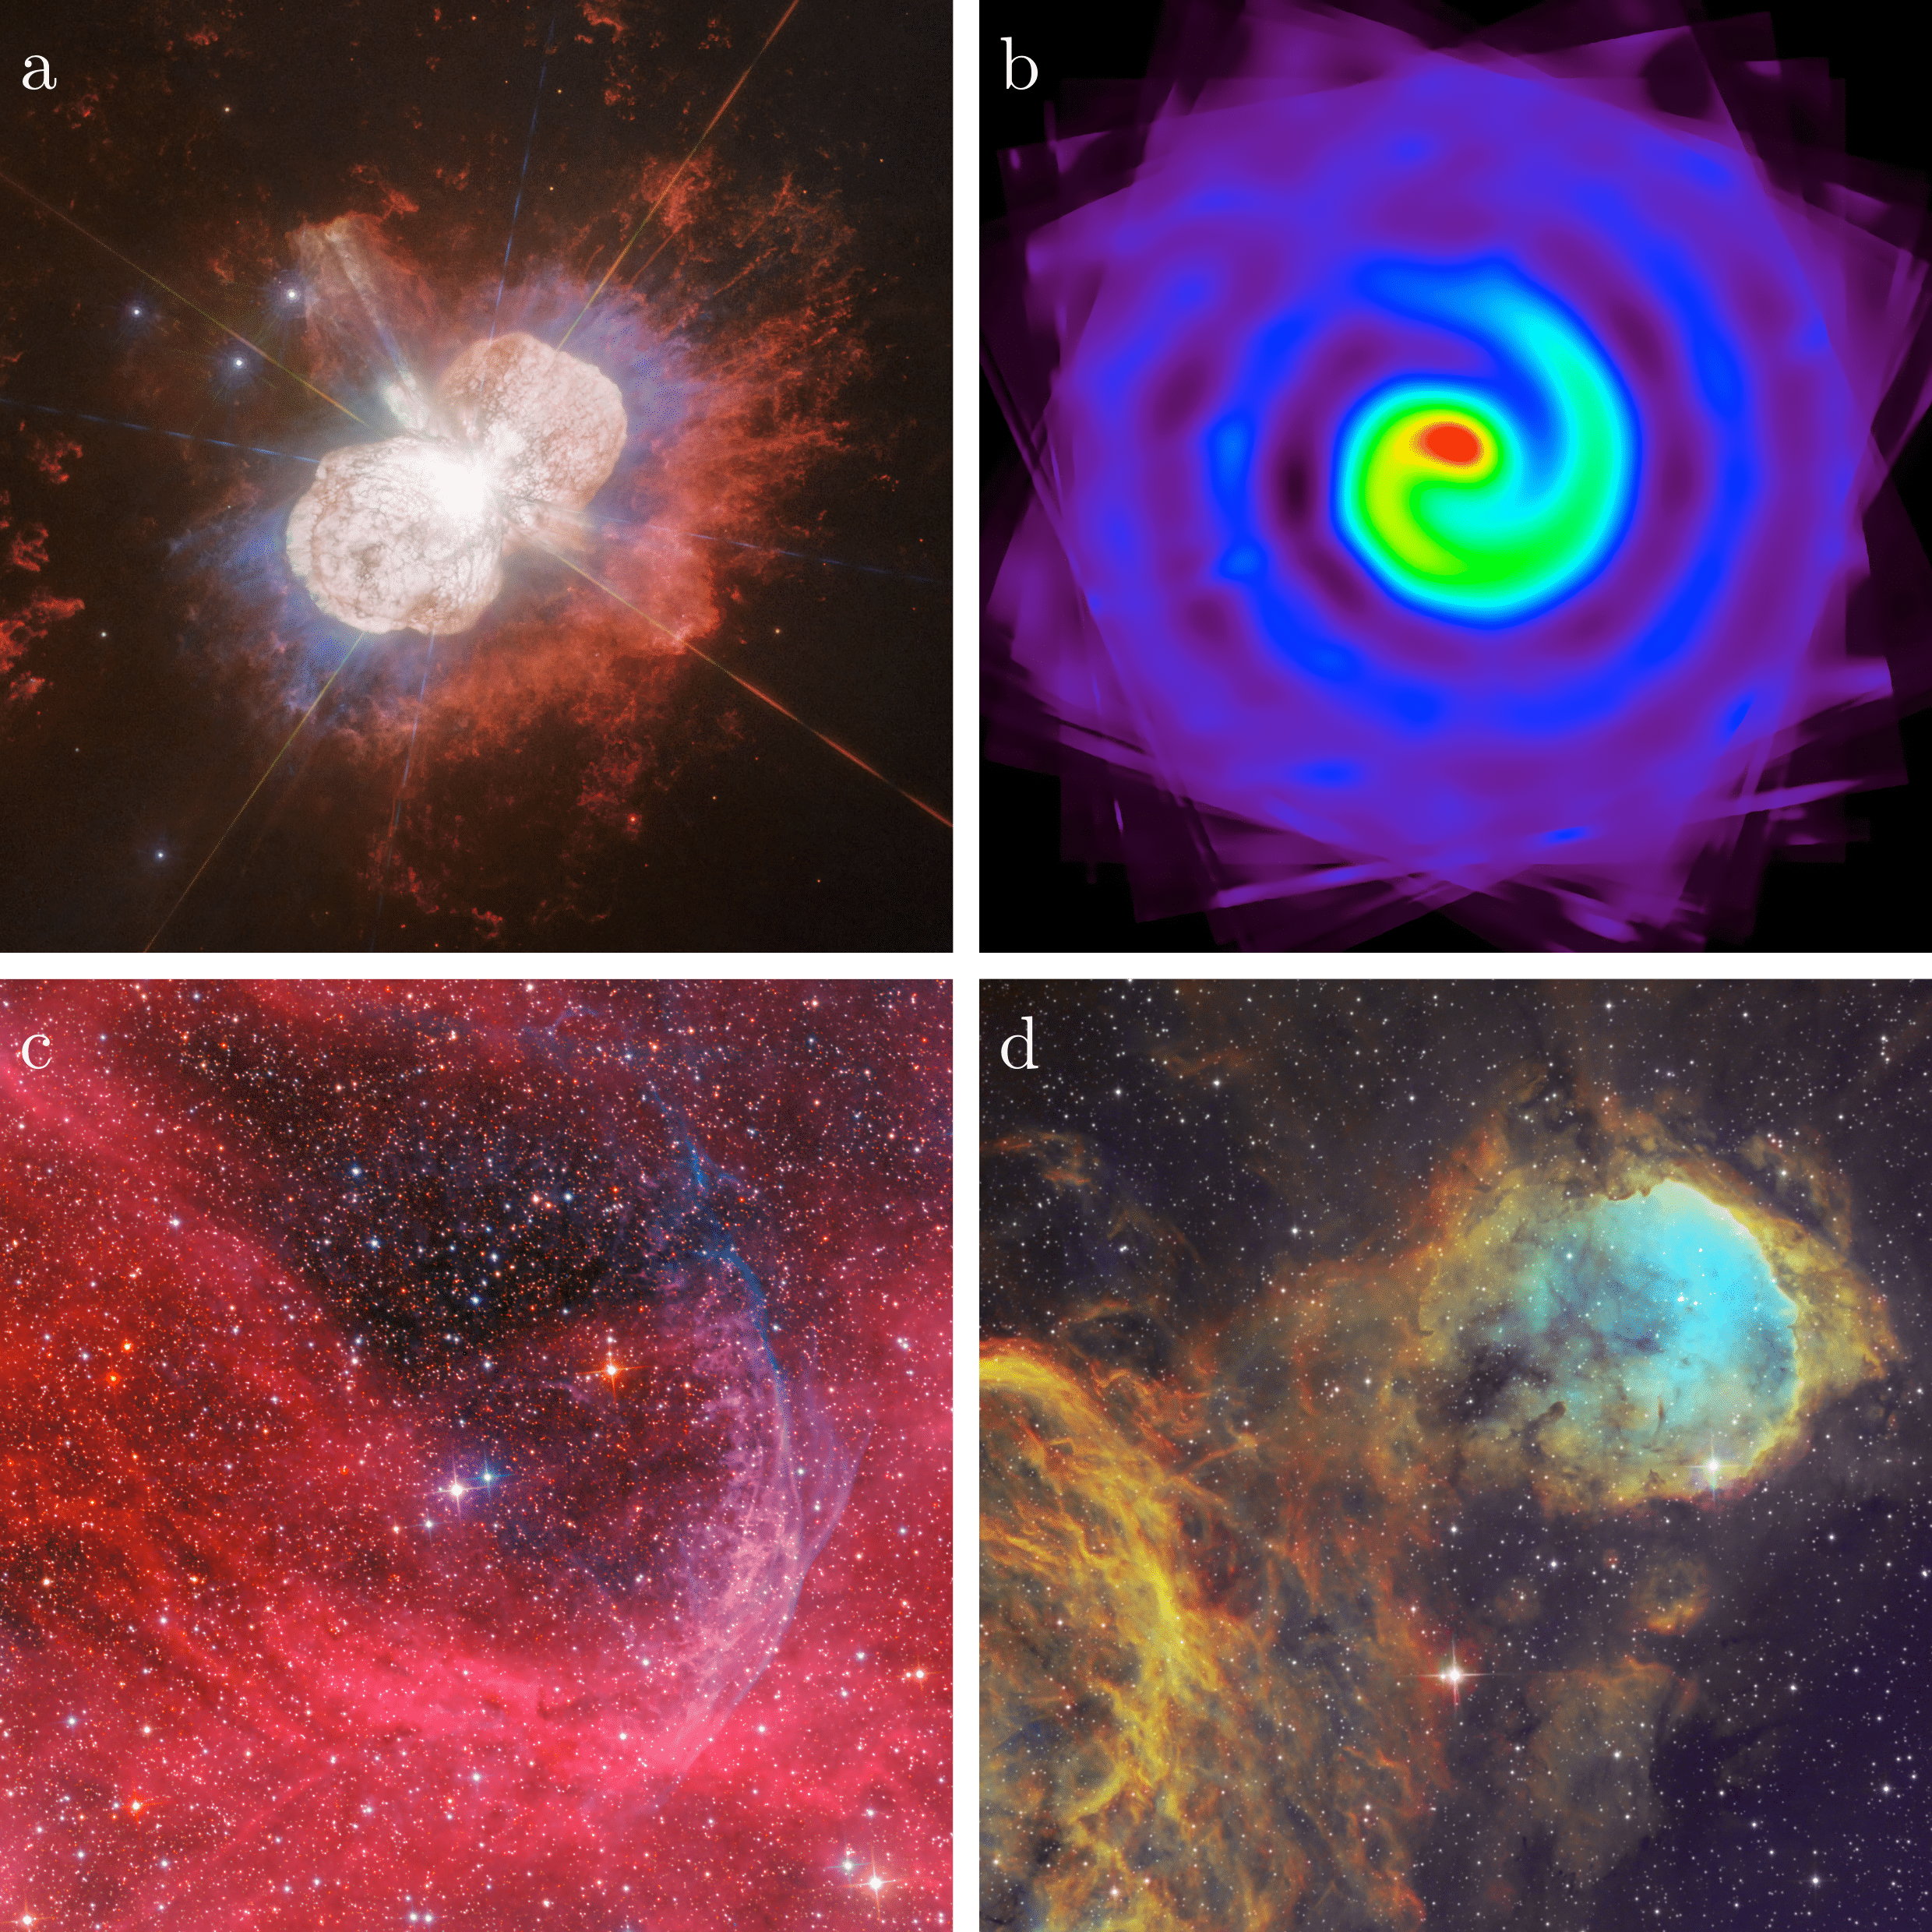
\includegraphics[width=5in]{assets/wolf-rayets/wolf-rayets.png}
  \caption[\emph{NASA APOD images of Wolf-Rayet and CWB systems}]{NASA Astronomy Picture of the Day (APOD) images of Wolf-Rayet and CWB systems. (a) The LBV+O system $\eta$ Carinae (\link{https://apod.nasa.gov/apod/ap190220.html}). (b) The persistent dust forming colliding wind binary (WCd) system WR 104 (\link{https://apod.nasa.gov/apod/ap140603.html}). (c) The WR134 ring nebula (\link{https://apod.nasa.gov/apod/ap120621.html}). (d) The Wolf-Rayet nebula surrounding WR23 (\link{https://apod.nasa.gov/apod/ap210208.html}). Wolf-Rayet and CWB systems are, without a doubt, some of the most striking systems in the galaxy.}
  \label{fig:cwbexamples}
\end{figure}

Colliding Wind Binary (CWB) systems are perhaps one of the most striking types of stellar system.
% Notes on beauty
Beauty, as they say, is in the eye of the beholder -- and nearly every astrophysicist believes that parts of their specialist subjects hold tremendous aesthetic qualities.
Figure \ref{fig:cwbexamples}, however, really does show off the intrinsic beauty of both Wolf-Rayet (WR) stars and CWB systems.

These systems can produce a variety of beautiful outbursts, from Wolf-Rayet nebulae to delicate interstellar dust clouds forming around them in the infrared.
The latter form either fine filaments, or pinwheels extending out for parsecs, with an enormous amount of structural variety.
On top of the visible and infrared, these systems are also visible from the radio to gamma rays, emitting copious amounts of radiation though both thermal and non-thermal mechanisms.

Massive stars have an incredibly outsized influence on their local interstellar medium (ISM).
Even in a single system, these stars produce winds capable of perturbing their local medium, forming pockets of high density material that can drive star formation, as well as ionising this medium, producing HII regions.
WR stars turn the metaphorical dial of this influence up to eleven, driving enormous quantities of hot, ionised wind into the ISM.
Massive stars literally tear themselves apart over a period of around 500,000 years, flinging many solar masses worth of material into space at an appreciable fraction of the speed of light.
These stars too, are destined to die in violent, chaotic, and beautiful\footnote{Provided you are not in the blast radius.} ways, such as supernovae and gamma-ray bursts (GRBs).

If these stars form a close binary with colliding winds we observe incredibly powerful shocks, as the mechanical energy equivalent to the luminance of a thousand suns acts on a region only a few solar radii in size.
This heats this wind collision region (WCR) to temperatures in excess of $10^8 \, \si{K}$ as these winds crash headlong into each other.
These systems are among the brightest continuous x-ray sources in the night sky (Fig. \ref{fig:intro-xray}), and provoked much scientific debate before the discovery of their true nature. 

\begin{figure}[ht]
  \centering
  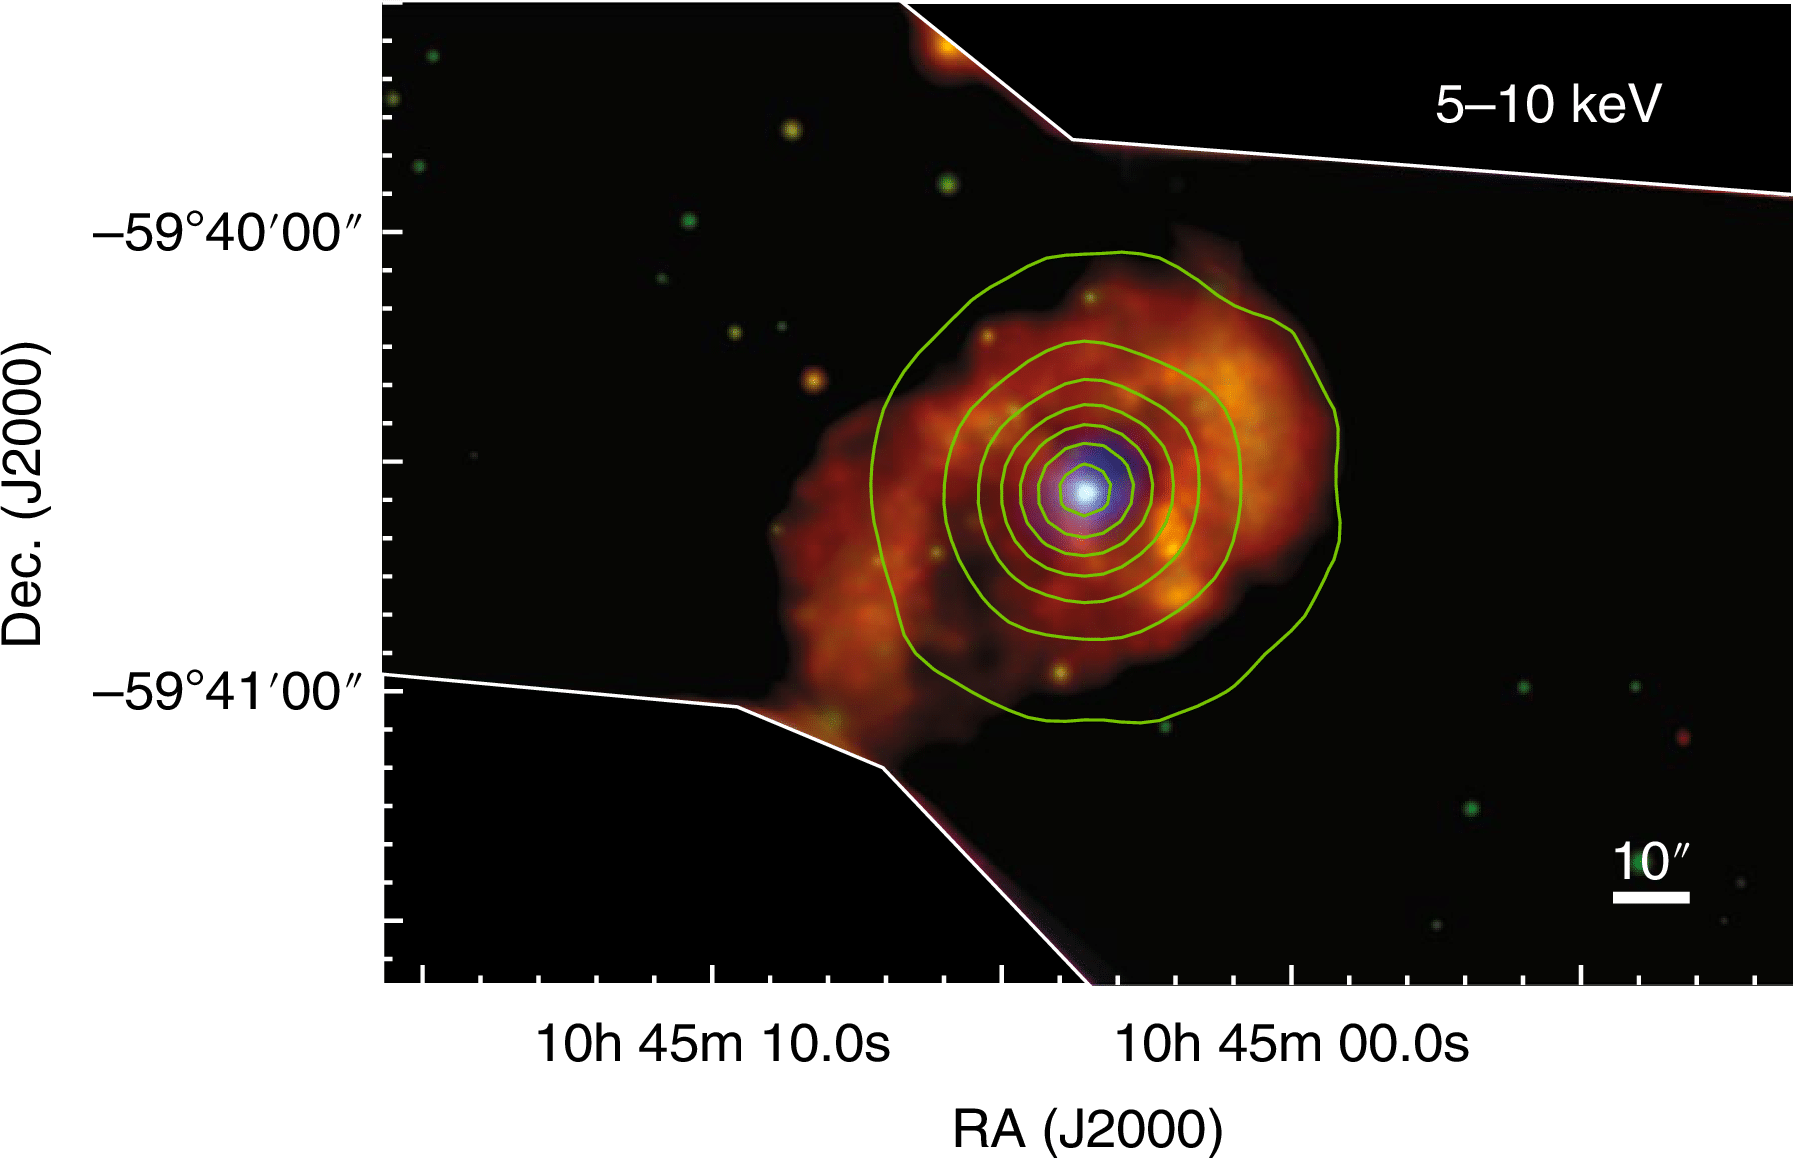
\includegraphics[width=4in]{assets/wolf-rayets/x-ray.png}
  \caption[\emph{Chandra \& NuSTAR imagery of $\eta$ Carinae \parencite{hamaguchiNonthermalXraysColliding2018}}]{Chandra x-ray imagery of $\eta$ Carinae at the soft x-ray minimum of 2009, with contours from the NuSTAR $5-10 \, \si{\kilo\electronvolt}$ x-ray band. CWB systems are incredibly bright in x-ray bands due to the powerful shock heating driving thermal x-ray processes. Image sourced from \textcite{hamaguchiNonthermalXraysColliding2018}.}
  \label{fig:intro-xray}
\end{figure}

However, a most puzzling question is how dust forms in certain CWB systems (which we refer to as WCd systems throughout this thesis).
These systems have violent shocks, incredibly high temperatures, and produce copious amounts of ionising radiation.
So how can it be that something as tenuous as interstellar dust can form?
The mechanisms behind formation and growth are extremely poorly understood, and as such we intend to glean some information on the mechanisms and yields of dust production processes in these systems.

\section{Motivation \& Goals}
\label{sec:projectgoals}

% Initial motivation
Dust formation in early-type star systems is a relatively poorly understood phenomenon.
As the grains should be readily destroyed by shocks and ionising radiation, nascent grain cores must require some form of shielding or rapid dust growth mechanisms in order to form larger grains.
% Point of dust formation
\note{
  We find that some of these binary systems can produce dust at similar rates to asymptotic giant branch stars ($\sim\SI{1e-5}{\solarmass\per\year}$ of dust, see \textcite{lauRevisitingImpactDust2020}).
  Though these systems are significantly rarer than AGB systems and do not inject as much dust into the interstellar medium when compared to individual supernova \parencite{draineInterstellarDustGrains2003}, the influence on their local stellar environment should not be discounted. 
  Furthermore, in the early universe when massive stars were more common these systems would have had more influence on the dust content of the galactic interstellar medium \parencite{morganDustFormationEarly2003}.
}
\note{We must also consider that dust} formation is vital for the formation of planets and complex organic molecules throughout the galaxy, so understanding the mechanisms behind its formation is of significant scientific interest.
% Stellar feedback and massive stars 
CWB systems are -- for a variety of reasons -- very difficult to both observe \emph{and} simulate.
WR CWB systems are quite distant, with the nearest systems being typically more than \SI{2}{\kilo\parsec} from Earth, making the wind collision region (WCR) very difficult to observe.
The WCR is also shrouded by dense stellar winds, occluding the shock region.
These systems are also comparatively rare, making it more difficult to typify these systems.
If we simulate these systems, we find other difficulties such as a requirement of 3D simulation in order to model orbital effects.
CWB systems also have a large variation in length scales that render the simulations very computationally challenging.

% Development of a dust model
The main goal of the project was to develop a dust model that was computationally inexpensive to implement, such that it could be included in large-scale numerical models.
% Broad outline of feature set, link to sections
This dust formation model\footnote{Christened \bidmas{}, or binary interaction dust model with accretion and sputtering.} was designed to be as modular as possible, and to be relatively straightforward to implement additional dust evolution mechanisms.
By the end of the project, dust evolution and destruction mechanisms were implemented, as was dust cooling through gas-grain collisional excitation.

% MOdel two types of system
The second goal of the project was to simulate a variety of WCd systems using this dust model running within a hydrodynamical simulation.
WCd systems can be sub-categorised by the time dependence of their dust formation:

\begin{itemize}
  \item ``Episodic'' systems that produce dust over a small section of their orbit. 
  \item ``Variable'' systems whose dust production varies significantly over their orbital period.
  \item ``Persistent'' systems whose dust did not vary significantly over the orbital period.
\end{itemize}

\noindent
% It was intended from the beginning of the project to observe at least two of these systems, with the work on each system constituting a journal paper.
% Overall, two such systems archetypes, variable and episodic, were simulated.
% Persistent dust forming systems -- WR98a
The first type of WCd system modelled was the variable dust forming system WR98a.
We found that this system was the easiest to simulate, due to its comparatively sedate winds and larger orbital spacing. 
% Parameter space search 
In addition to simulating a system with parameters similar to WR98a, a parameter space search was conducted using WR98a as a baseline: wind properties predicted to be influencing the dust production rate were varied, in order to understand their effects.
% Episodic dst forming systems -- WR140
The episodic dust forming system WR140 was also simulated, whose dust formation is theorised to be due to its high orbital eccentricity.
This was a more complex affair, as the system was far more complex to simulate than WR98a.
This section of the project had to be partially truncated due to time constraints, and a partial orbit of the system near periastron was opted for in lieu of a full orbit of the system.

% Missed opportunities, time limitations
% It should be noted that there were a number of technical difficulties throughout the project, and as such, a lot of the project was conducted on a very time-constrained basis.
Whilst the main goals of the project were completed, there is still much that is not understood about dust formation in these systems.
Development of a more complex model, as well as synthetic astronomical imaging through radiative transfer models were topics considered for later stages of this project but could not be accomplished due to time.
However, these projects present interesting avenues of future research.
Other wind features, such as radiative line driving, would also be included in future models, in order to understand their role in dust formation, and how they influence grain growth and dust yields.
Furthermore, simulation of other systems, such as the WR+WR systems WR70-16 ``Apep'' and WR48a would be interesting follow-up simulation targets.

\section{Thesis Structure}

The structure of this thesis could be described as somewhat unconventional, this is because of two primary reasons:

\begin{itemize}
  \item Difficulties in the early and middle sections of the project.
  \item The field itself requiring a significant degree of explanation.
\end{itemize}

\noindent
Throughout the \nth{2} and \nth{3} years of this PhD, there were many issues with getting this project to even progress at all.
This was mostly due to being unable to get the original hydrodynamical code used in this experiment to work with our dust model (Section \ref{sec:mgcode}).
This code was ultimately abandoned by the \nth{3} year and replaced with a more modern and easier to develop code, \athena{} (Section \ref{sec:athenapp}).
Additionally the outbreak of a global pandemic resulted in a stalling of some aspects of the work in the thesis.
This meant that there was a lot of time to develop the codebase and theorise on the nature of these systems, but much of the actual data collection was performed in the last few months of the project.
As such, there is a great deal of discussion of the background and methodology, and an enormous amount of discussion on the future of this particular field.
While the primary objectives of this PhD were achieved, many aspects of this thesis that were planned out at the start of the project were unfortunately truncated or removed.
This was extremely disappointing, of course, but I hope to continue work on this field outside of this PhD, and develop a more advanced dust model for numerical simulation.

% Two introductory sections
Astrophysical fluid dynamics straddles two particularly complex fields: physics and computer science.
% Unfortunately universities don't award two PhDs for work involving this subject, instead we have to discuss these two fields at great length.
Because of this, the first two chapters of this thesis are both background chapters\footnote{A friend of mine wrote their thesis on computational biophysics that had not one, not two, but \emph{three} background chapters, so it could be worse.}.
In Chapter \ref{ch:background} we discuss the physics of massive stars and dust, before synthesising these two sections in order to discuss dust producing CWB systems.
In Chapter \ref{ch:numsim} we discuss the underlying principles of numerical simulation, and discuss our model, from the choice of numerical code to the underlying mechanisms and methodology.
% Paper chapters
Afterwards, we will move on to Chapters \ref{chap:parameterspace} \& \ref{ch:wr140}.
These chapters have been adapted from two papers written concurrently with this thesis:

\begin{enumerate}
  \item \emph{\firstpapertitle} \parencite{eatsonExplorationDustGrain2022}.
  \item \emph{\secondpapertitle} \parencite{eatsonExploringDustGrowth2022}.
\end{enumerate}

\noindent
These chapters serve to provide more concise explanations of our work, while also providing the results of this research, particularly dust formation rates of both persistent and episodic WCd systems.
Finally, we will conclude with some remarks on future work that could be performed in this field, as well as with some observations made over the course of this project.